\documentclass{beamer}
\usepackage{multimedia}
\usepackage[comma,numbers,compress,square]{natbib}
\usepackage{listings}
\usetheme{polymtl}
\title{BittyBuzz}
\subtitle{Buzz for microcontrollers}
\author{Emir K. Belhaddad, Anthony Dentinger}
\date{\today}

\graphicspath{{resources/}}
\definecolor{darkorange}{RGB}{230,102, 0}
\newcommand{\tabitem}{~~\llap{\color{darkorange}\textbullet}~~}

\AtBeginSection[]
{
	\begin{frame}
	\frametitle{Content}
	\tableofcontents[currentsection]
	\end{frame}
}


% ========================================
% =               DOCUMENT               =
% ========================================

\begin{document}
	
	% ----------------------------------------
	% -                 CODE                 -
	% ----------------------------------------
	% Doing it this way is the only way I found to insert code blocks
	
	\defverbatim[colored]\buzzCClosure{
		\begin{lstlisting}[language=C,linewidth=5cm,basicstyle=\ttfamily\scriptsize,keywordstyle=\color{blue}]
int buzz_c_closure(buzzvm_t vm) {
  // Error if not passed 1 param.
  buzzvm_lnum_assert(vm, 1);

  // Take int value of param.
  buzzvm_lload(vm, 1);
  int16_t param1 =
    buzzvm_stack_at(vm, 1)->i.value;
  buzzvm_pop(vm);
	
  buzzobj_t result;
  // Compute result...

  buzzvm_push(result);
  return buzzvm_ret1(vm);
}
		\end{lstlisting}
	}
	
	\defverbatim[colored]\bittybuzzCClosure{
		\begin{lstlisting}[language=C,basicstyle=\ttfamily\tiny,keywordstyle=\color{blue}]
void bbz_c_closure() {
  // Error if not passed 1 param.
  bbzvm_assert_lnum(1);

  // Take int value of param.
  int16_t param1 =
    bbzheap_obj_at(
      bbzvm_locals_at(1))->i.value;


  bbzheap_idx_t result;
  // Compute result...

  bbzvm_push(result);
  bbzvm_ret1();
}
		\end{lstlisting}
	}

	% ----------------------------------------
	% -                SLIDES                -
	% ----------------------------------------
	
	\begin{frame}
		\titlepage
	\end{frame}
	\begin{frame}
		\frametitle{Introduction}
		\begin{itemize}
			\item Buzz: \textbf{Description of collective swarm behavior} with both top-down and bottom-up approaches \cite{buzz_arxiv}. Details of information propagation are hidden.
			\item Swarm intelligence and behavior require large numbers of robots with limited resources $\Rightarrow$ results must be achieved with the \textbf{cheapest robots possible}.
		\end{itemize}

		\centering \Large
		\textbf{How cheap can Buzz go?}
	\end{frame}
	\begin{frame}
		\frametitle{Introduction}
		\textbf{BittyBuzz}: Reimplementation of \textbf{Buzz for microcontrollers}. Designed for very cheap robots with extreme resource constraints.\\
		~\\
		Currently, only implementation is for \textbf{Kilobots}, inexpensive robots designed by Harvard to swarm in the thousands \cite{kilobot_paper}.
		\begin{figure}
			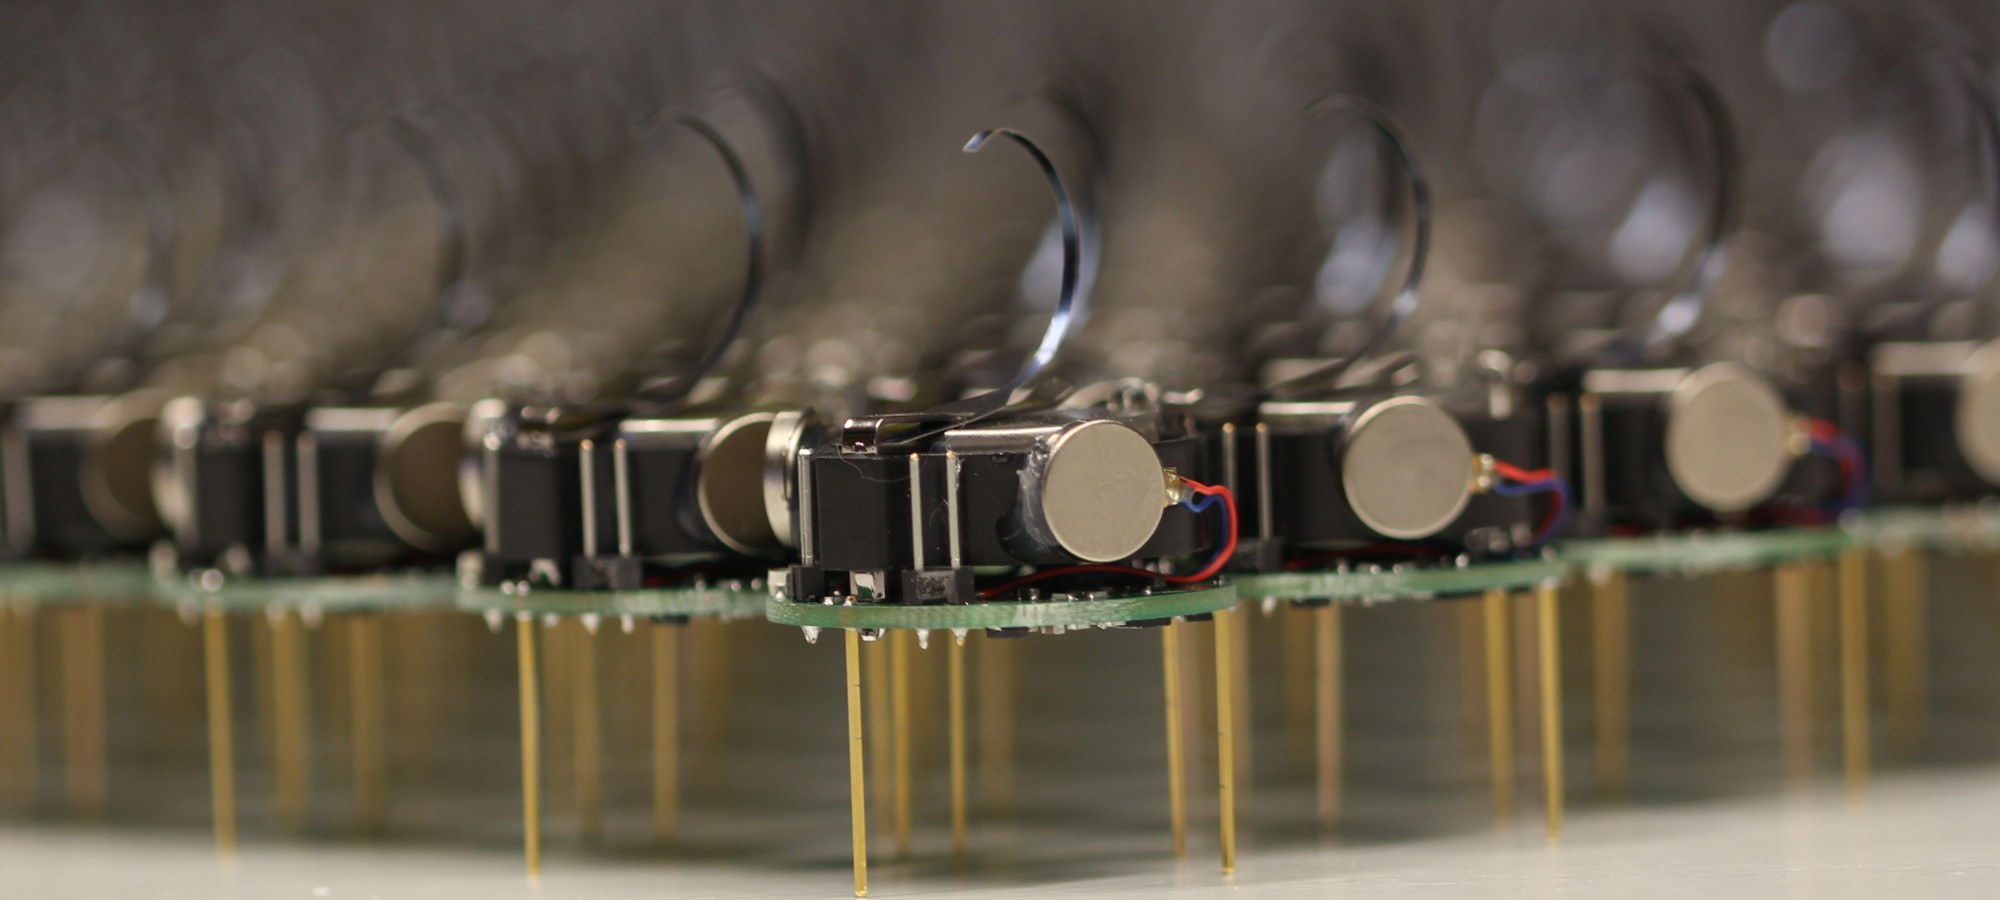
\includegraphics[width=0.5\textwidth]{swarm2}
			\caption{\label{figure:Kilobots}Fig. \ref{figure:Kilobots}: A Kilobot Batalion \cite{kilobot_pic}}
		\end{figure}
	\end{frame}
	\begin{frame}
		\frametitle{Outline}
		\tableofcontents
	\end{frame}
	\section{Overcoming resource limitations}
	\begin{frame}{Resource comparison}
		Let us start by comparing the 2 targeted platforms:
		\begin{itemize}
			\item {\bfseries Khepera IV}: Robot with a system able to support Buzz.
			\item {\bfseries Kilobot}: Robot with \textbf{very} little resources available.
		\end{itemize}
		\begin{table}
			\begin{tabular}{l|c|c}
				& Khepera IV        & Kilobot\\
				\hline
				Processor         & 32-bits @ 800 MHz & 8-bits @ 8 MHz\\
				Flash             & 512 MB (+ 4 GB)   & 32 KB\\
				RAM               & 512 MB            & 2 KB\\
				Payload bandwidth & $\sim$ 1 MB/s \footnote{Assuming CCK modulation scheme} \cite{khepera_wifi}  & 350-450 B/s\\
				Packet drops      & None with TCP/IP  & $\approx$ 50\%
			\end{tabular}
			\caption{
				\label{table:khepera kilobot comparison}Table \ref{table:khepera kilobot comparison}: Resource comparison between the Khepera IV and Kilobot robots \cite{khepera_specs}}
		\end{table}
	\end{frame}
	\subsection{Dynamic memory management}
	\begin{frame}{Dynamic memory management}
		\begin{itemize}
			\item Internal pre-allocated heap % Fixed size
			\item 3 sections: Objects, Segments and Unclaimed
			\item All objects have 2 bytes payload and 1 byte meta-data
			% ... which allows for a ...
			\item Simple GC algorithm
		\end{itemize}
		\begin{figure}
			\centering
			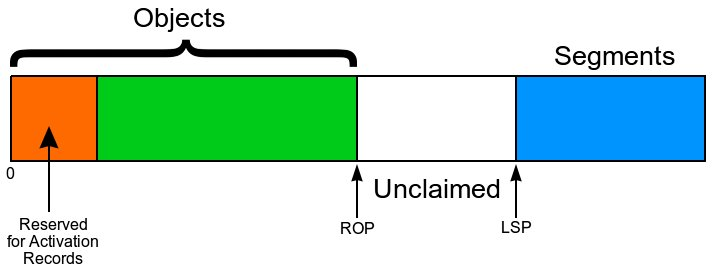
\includegraphics[width=\linewidth]{schematic_heap.jpg}
			\caption{
				\label{figure:heap sections}Fig. \ref{figure:heap sections}: Section placement in the heap}
		\end{figure}
	\end{frame}
	\subsection{Point on Optimizations}
	\begin{frame}{Point on Optimizations}
		Some optimizations made on BittyBuzz, grouped by what they optimize:
		\begin{table}
			\begin{tabular}{l|l|l}
				RAM & Flash & Bandwidth\\
				\hline
				\tabitem Closures & \tabitem Function vs Macros & \tabitem Sorted neighbors\\
				\tabitem 2B payload & \tabitem Optimized loops & \tabitem Ring-buffers\\
				\tabitem Unique alloc & \tabitem Translated bytecode &\\
				\dots & \dots & \dots
			\end{tabular}
			\caption{
				\label{table:Optimizations}Table \ref{table:Optimizations}: Some of the optimizations made to BittyBuzz}
		\end{table}
	\end{frame}
	\section{$BittyBuzz \approx Buzz$}
	\begin{frame}
		Differences between BittyBuzz and Buzz are minimal per design choice. Nonetheless, \textbf{what differences have resulted from these limitations?}\\
		\[BittyBuzz - Buzz =~?\]
		Theorem (accepted):
		\begin{align}
		\begin{split}
		BittyBuzz - Buzz = ~&\Delta Architecture + \Delta (Buzz~features)\\
		+ &\Delta (Closure~definitions) + (small~improvements)
		\end{split}
		\end{align}
	\end{frame}
	\subsection{Architecture}
	\begin{frame}
		\frametitle{Architecture}
		Microcontrollers with no OS $\Rightarrow$ existence of platform-dependant operations.\\
		Out of the box, BittyBuzz thus has \textbf{two layers of implementation}:
		\begin{itemize}
			\item Higher-level "core" layer for \textbf{platform-independant operations} (VM bytecode execution, definition of \texttt{swarm}, \texttt{stigmergy}, ...).
			\item Thin, lower-level robot layer for \textbf{platform-dependant operations} (fetching bytecode, displaying errors, sending and receiving packets, ...). Must be implemented for each robot.
		\end{itemize}
		This is contrary to Buzz, which only contains the "core" layer, and requires implementation for each platform.
	\end{frame}
	\subsection{Buzz features}
	\begin{frame}
		\frametitle{Buzz features}
		Consistency with Buzz has been a key factor to the development choices, however \textbf{some features still have limitations}. Examples:
		\begin{itemize}
			\item Only one \texttt{stigmergy} allowed ;
			\item \texttt{stigmergy} topic must be a string (currently, but can be overcome) ;
			\item \texttt{swarm} IDs range from 0 to 7.
		\end{itemize}
	\end{frame}
	\textsl{\textsl{}}\subsection{Closure definitions}
	\begin{frame}
		\frametitle{Closure definitions}
		Buzz C closures allow a user to call a C function from the Buzz side. Making them in BittyBuzz is also very similar.\\
		~\\
		\begin{figure}
			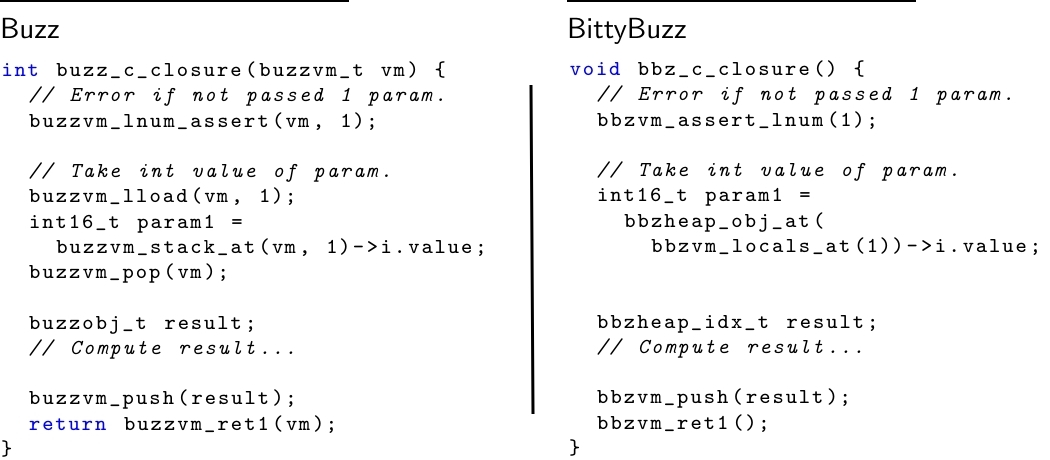
\includegraphics[width=1\textwidth]{ClosureDefinitions}
			\caption{\label{figure:C Closures}Fig. \ref{figure:C Closures}: C Closures in Buzz vs. BittyBuzz}
		\end{figure}
	\end{frame}
	\section{Project results}
	\begin{frame}
		Made several demo Buzz scripts to test BittyBuzz on real Kilobots.
		We'll present 3 of them in the next slides.\par
		\centering
		\LARGE Enjoy!
	\end{frame}
	\subsection{Distance Gradient Algorithm}
	\begin{frame}
		\begin{figure}
			\lstinputlisting[language=Python,basicstyle=\tiny,showspaces=false,breaklines=true,keywordstyle=\color{darkorange},commentstyle=\color{gray}]{resources/gradient.bzz}
			\caption{
				\label{figure:gradient code}Fig. \ref{figure:gradient code}: Distance gradient source code}
		\end{figure}
	\end{frame}
	\begin{frame}{Distance Gradient Algorithm}
		\centering
		\movie[width=\linewidth,height=0.5625\linewidth,showcontrols,start=64s,poster]{distance gradient demo}{resources/gradient.mov}
	\end{frame}
	\subsection{Stigmergy Demo}
	\begin{frame}
		\begin{figure}
			\lstinputlisting[language=Python,basicstyle=\tiny,showspaces=false,breaklines=true,keywordstyle=\color{darkorange},commentstyle=\color{gray}]{resources/stigmergy.bzz}
			\caption{
				\label{figure:stigmergy code}Fig. \ref{figure:stigmergy code}: Stigmergy demo source code}
		\end{figure}
	\end{frame}
	\begin{frame}{Stigmergy Demo}
		\centering
		\movie[width=\linewidth,height=0.5625\linewidth,showcontrols,start=64s,poster]{distance gradient demo}{resources/stigmergy.mov}
	\end{frame}
	\subsection{Swarm Demo}
	\begin{frame}
		\begin{figure}
			\lstinputlisting[language=Python,basicstyle=\tiny,showspaces=false,breaklines=true,keywordstyle=\color{darkorange},commentstyle=\color{gray}]{resources/swarm.bzz}
			\caption{
				\label{figure:swarm code}Fig. \ref{figure:swarm code}: Swarm demo source code}
		\end{figure}
	\end{frame}
	\begin{frame}{Swarm Demo}
		\centering
		\movie[width=\linewidth,height=0.5625\linewidth,showcontrols,start=64s,poster]{distance gradient demo}{resources/swarm.mov}
	\end{frame}
	\section{Future work}
	\begin{frame}{Future work}
		So that's it?\\
		~\\
		No. There is still more work to be done for BittyBuzz:
		\begin{itemize}
			\item Implementation of \textbf{BittyBuzz for zooids}.
			\item Keep BittyBuzz up to date with new Buzz features.
			\item Many, many general improvements.
			\item Conduct \textbf{research projects using BittyBuzz}.
			\item \textbf{Write an IEEE paper} on BittyBuzz.
		\end{itemize}
		~\\
		\begin{quote}
			When you're finished changing, you're finished. -- Benjamin Franklin
		\end{quote}
	\end{frame}
	\begin{frame}{Concluding words}
		\section{}
		All in all, BittyBuzz:
		\begin{itemize}
			\item Reworks (and somewhat improves) Buzz, targetting the \textbf{specific limitations of inexpensive robots using microcontrollers};
			\item Attempts to \textbf{behave as Buzz} whilst allowing for easy extension to new robots ;
			\item Can implement simple swarm behaviors \textbf{on Kilobots}.
		\end{itemize}
	\end{frame}
	\begin{frame}{Concluding words (continued)}
		\begin{quote}
			So long, and thanks for all the fish!
		\end{quote}
		\begin{figure}
			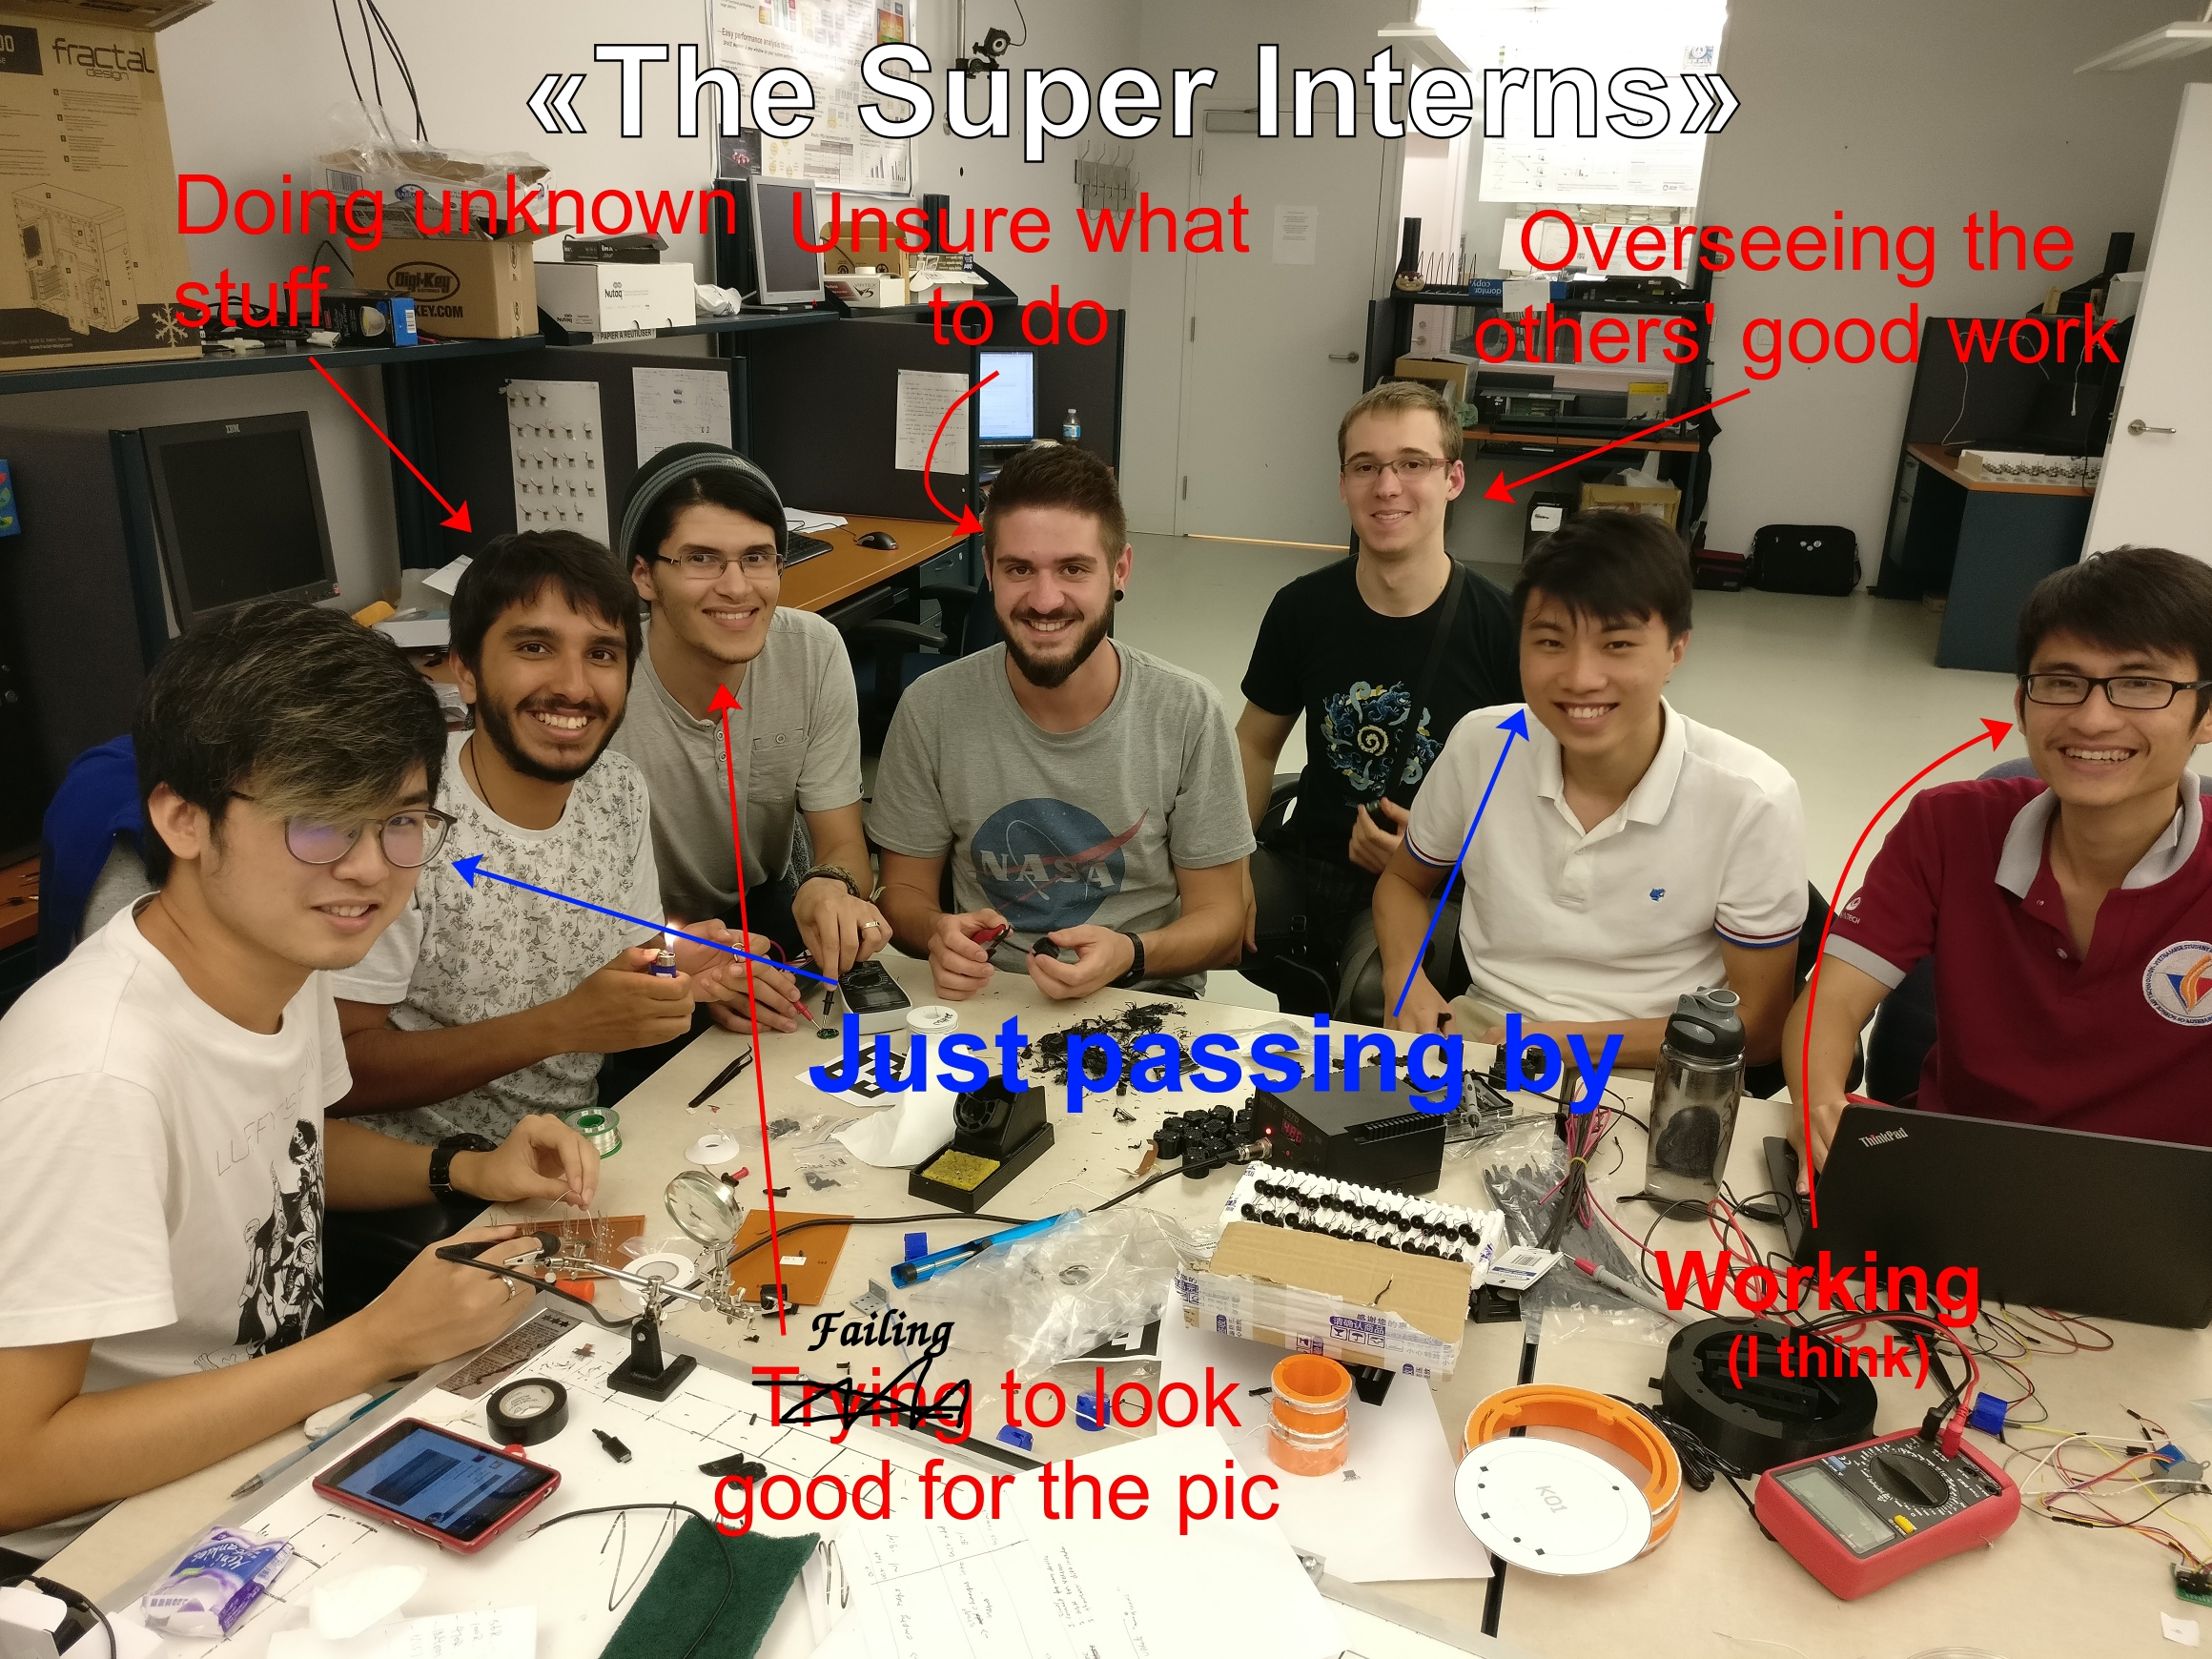
\includegraphics[width=0.7\textwidth]{the_great_interns}
			\caption{\label{figure:The Great Interns}Fig. \ref{figure:The Great Interns}: "And now, for something completely different..."}
		\end{figure}
	\end{frame}
	\begin{frame}[allowframebreaks]
		\frametitle{References}
		\bibliographystyle{IEEEtran}
		\bibliography{refs}
	\end{frame}
\end{document}
